\documentclass[oneside,a4paper]{amsart}
%\usepackage{maa-monthly}
\usepackage{gauss-bonnet}
\usepackage{amsmath, amsfonts}
\usepackage{amsthm}
\newtheorem{exer}[thm]{Exercise}
\newtheorem{prob}[thm]{Problem}
%\usepackage[russian,english]{babel}
%\usepackage[utf8]{inputenc}

\begin{document}

\title{An exercise on the comparison theorem}
\author{Anton Petrunin and Sergio Zamora Barrera}
%\address{Anton Petrunin,  Math. Dept., PSU, University Park,  PA 16802, USA.}
%\address{aqp6@psu.edu}
%\address{Sergio Zamora Barrera,  Math. Dept., PSU,University Park,  PA 16802, USA.}
%\address{sxz38@psu.edu}

\keywords{discrete minimal surface, polyhedral surface, area minimizing surface, minimal surface.}
\maketitle


A famous interpretation of curvature is the following: ``In the presence of positive curvature, triangles are fat, and in the presence of negative curvature, triangles are thin.'' This can be stated more precisely (see Theorems \ref{B} and \ref{C}). Here we briefly discuss some consequences of this phenomenon in how geodesics in surfaces intersect.


\begin{figure}[h]
\begin{center}
\includegraphics[scale=0.9]{P1.jpg}\\
\end{center}
\end{figure}



\begin{thm}\label{A}
Let $\Sigma \subset \mathbb{R}^3$ be a smooth complete simply connected surface with Gaussian curvature $K : \Sigma \to \mathbb{R}$.
\begin{itemize}
\item If $K\leq 0$, then $\Sigma$ is diffeomorphic to $\mathbb{R}^2$.
\item If $K \geq 0$, then $\Sigma$ is diffeomorphic to $\mathbb{S}^2$ or $\mathbb{R}^2$. In the former case, $\int_{\Sigma} K dA = 4 \pi$ and we say that $\Sigma$ is closed. In the latter case, $\int_{\Sigma} K dA \leq 2 \pi$, and we say that $\Sigma$ is open.
\end{itemize}
\end{thm}

\section*{Comparison Theorems}

Throughout this note, we will call a smooth complete simply connected surface $\Sigma \subset \mathbb{R}^3$ with either $K \geq 0$ or $K \leq 0$ an \textit{Alexandrov surface}. As a consequence of Theorem \ref{A} and the Jordan Curve Theorem, every simple closed curve $\gamma$ in an Alexandrov surface $\Sigma$ separates it in two regions, from which at least one of them is homeomorphic to a disk $D$ with $\partial D = \gamma$.



\begin{figure}[h]
\begin{center}
\includegraphics[scale=0.9]{P2.jpg}\\
\end{center}
\end{figure}

We define a \textit{polygon} in a smooth surface $\Sigma \subset \mathbb{R}^3$ to be a subset $P$ homeomorphic to a closed disk with $\partial P$ a piecewise smooth curve such that each smooth piece (called \textit{side}) is a geodesic. A polygon of 3 (resp. 1, 4, or 5) sides will be called a \textit{triangle} (resp. \textit{monogon}, \textit{cuadrangle,} or \textit{pentagon}).


\begin{figure}[h]
\begin{center}
\includegraphics[scale=0.9]{P3.jpg}\\
\end{center}
\end{figure}


\begin{thm}\label{B}
Let $P$ be a polygon of $n$-sides in a smooth surface, and let $\Theta$ be the sum of the interior angles of $P$. Then
$$  \Theta = (n-2) \pi + \int_P K dA. $$
\end{thm}

\begin{thm}\label{C}
Let $P$ be a triangle in an Alexandrov surface with vertices $A, B, C$ and assume each side is a shortest path between its endpoints. Let $\alpha , \beta , \gamma$ be the interior angles of $P$ at $A,B,C$, respectively. Construct a triangle $A'B'C'$ in $\mathbb{R}^2$ with equal corresponding sidelengths as $P$ and let $\alpha ' ,\beta ' , \gamma ' $ be its interior angles at $A' , B'  , C' $, respectively.
\begin{itemize}
\item If $K \geq 0$, then $\alpha \geq \alpha '$, $\beta \geq \beta '$, $\gamma \geq \gamma '$.
\item If $K \leq 0$, then $\alpha \leq \alpha '$, $\beta \leq \beta '$, $\gamma \leq \gamma '$.
\end{itemize}
\end{thm}

\section*{Geodesic Configurations}

Using these two theorems, it is not hard to deduce that some geodesic configurations cannot occur in certain Alexandrov surfaces.

\begin{exer}
Let $\Sigma\subset \mathbb{R}^3$ be an Alexandrov surface $K \leq 0$ and let $D\subset \mathbb{R}^2$ be the unit disk.
\begin{enumerate}
\item \label{i} Show that a geodesic cannot self intersect.
\item \label{ii} Show that two distinct geodesics cannot intersect twice.
\item Show that for any finite set of simple curves $\gamma_1 , \ldots , \gamma _{\ell} : [0,1] \to D$ with $\gamma_i^{-1}(\partial D) = \{ 0,1 \}$ for each $i$, and $\vert \gamma_i ([0,1]) \cap \gamma_j ([0,1]) \vert \in \{ 0,1 \}$ for $i \neq j$, there is a homeomorphism $int (D) \to \mathbb{H}$ from the interior of $D$ to the hyperbolic plane such that $\phi \circ \gamma_i \vert_{(0,1)}$ is a geodesic for each $i$. In other words, \ref{i} and \ref{ii} represent the only obstructions in which geodesics could potentially intersect in an Alexandrov surface with $K \leq 0$.
\end{enumerate}
\end{exer}


\begin{figure}[h]
\begin{center}
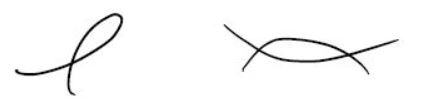
\includegraphics[scale=0.9]{P4.jpg}\\
\end{center}
\end{figure}

If $K \geq 0$, the situation is way more interesting and direct applications of Theorems \ref{B} and \ref{C} are usually not enough to understand how geodesics can intersect.

\begin{exer}
Let $\Sigma$ be an Alexandrov surface with $K \geq 0$. 
\begin{itemize}
\item Show that no geodesic segment in $\Sigma $ can have the following intersection configuration.

\begin{figure}[h]
\begin{center}
\includegraphics[scale=0.9]{P5.jpg}\\
\end{center}
\end{figure}

\item Show that if $\Sigma$ is open, a geodesic segment cannot have the intersection patterns from the figures below.

\begin{figure}[h]
\begin{center}
\includegraphics[scale=0.5]{P6.jpg}\\
\end{center}
\end{figure}

\item Give an example of an open Alexandrov surface and a geodesic in it that self intersects infinitely many times. Try to describe such intersection configuration.
\end{itemize}
\end{exer}

We now provide a couple of examples of how to exploit Theorems \ref{B} and \ref{C} in order to understand geodesic intersection patterns.

\begin{prob}\label{D}
Let $\Sigma$ be a closed Alexandrov surface with $K > 0$. Then no closed geodesic can have the following intersection pattern.
\end{prob}


\begin{figure}[h]
\begin{center}
\includegraphics[scale=0.9]{P7.jpg}\\
\end{center}
\end{figure}


\textit{Solution:} Let $\alpha, \beta, \gamma$ the angles labeled in the figure. Since they are the interior of a triangle in a surface with $K > 0$, $\alpha + \beta + \gamma > \pi$ by Theorem \ref{B}. Let $P_A, P_B, P_C$ be the monogons with interior angles $\alpha, \beta, \gamma$, respectively. By Theorem \ref{B},
\begin{eqnarray}
\int_{\Sigma }K dA & > & \int_{P_A}K dA + \int_{P_B}K dA + \int_{P_C}K dA \\
& = & (\pi + \alpha ) + (\pi + \beta ) + (\pi + \gamma )\\
& > & 4 \pi ,
\end{eqnarray}
contradicting Theorem \ref{A}.

Note that Problem \ref{D} is not true if one only assumes $K \geq 0$ instead of $K > 0$. An example could be guessed by taking the boundary surface of a thin triangular prism and smoothing it out a little.


\begin{figure}[h]
\begin{center}
\includegraphics[scale=0.9]{P8.jpg}\\
\end{center}
\end{figure}

\begin{prob}
Let $\Sigma$ be a closed Alexandrov surface with $K \geq 0$. Then no closed geodesic an have the following intersection pattern.
\end{prob}

\begin{figure}[h]
\begin{center}
\includegraphics[scale=0.9]{P9.jpg}\\
\end{center}
\end{figure}

\textit{Solution:}  Arguing by contradiction, suppose that $\Sigma$ contains such a geodesic $\gamma$;
 we label the arcs and angles as on the left diagram.

%\begin{figure}[!ht]
%\begin{minipage}{.38\textwidth}
%\centering
%\includegraphics{mppics/pic-472}
%\end{minipage}\hfill
%\begin{minipage}{.58\textwidth}
%\centering
%\includegraphics{mppics/pic-473}
%\end{minipage}
%\end{figure}


Applying Theorem \ref{B} to the quadrangle $xcab$ and the pentagon $azbcy$, we get respectively,
\[2\cdot\alpha\le\beta+\gamma
\qquad\text{and} \qquad
2\cdot\beta+2\cdot \gamma\le\pi+\alpha.\leqno(\asterism)\]
It follows that $\alpha \le\tfrac \pi 3$.


Consider the part of the geodesic $\gamma$ without the arc~$a$.
It cuts from $\Sigma$ a pentagon $\Delta$ with sides and angles shown on the diagram on the right.

%\begin{wrapfigure}{r}{50 mm}
%\vskip-0mm
%\centering
%\includegraphics{mppics/pic-474}
%\vskip8mm
%\end{wrapfigure}

Since small segments of any geodesic on $\Sigma$ are length minimizing, we can add additional vertices to the sides of $\Delta$ so that each side becomes length-minimizing.
Choose a vertex $v$ and subdivide $\Delta$ into triangles by joining $v$ to other vertices of the broken geodesic.

Consider a model triangle for each triangle in the subdivision so that they share sides as in $\Delta$.
By the comparison inequality $({*}{*})$, the angles of the model triangles do not exceed the corresponding angles of the original triangle.
Therefore the model triangles form a plane pentagon $\tilde\Delta$ with convex polygonal sides.
Moreover its angles do not exceed the corresponding angles of $\Delta$.

%\begin{wrapfigure}{r}{50 mm}
%\vskip-4mm
%\centering
%\includegraphics{mppics/pic-500}
%\vskip0mm
%\end{wrapfigure}

It remains to show the described plane polygon does not exist.
Let us orient its  sides counterclockwise;
denote the obtained vectors by $s_1,\dots,s_k$.

On the other hand, the conditions on the angles of polygons imply that the vectors $s_i$ point in the complement of white sectors shown with angles marked on the diagram.
The sum of magnitudes of the vectors in each black sector is also marked.
Let $v$, $v'$, $w$, $w'$ be the marked unit vectors;
set $r=v+v'+w+w'$.
Observe that $(\asterism)$ implies that $r\ne 0$,
and, moreover, 
\[\langle r,s_1\rangle+\dots+\langle r,s_k\rangle>0,\]
but  $s_1+\dots+s_k=0$ --- a contradiction.


{\sloppy
\printbibliography[heading=bibintoc]
\fussy
}

\end{document}
